\documentclass[12pt, openany]{book}

% This is all the packages and settings and so on.
% It is using custom fonts that needs to be installed on the computer. If they are not present, they have to be added manually.
\input{setup/settings.tex}

% Defining files for bibliography
%\addbibresource{ref.bib}
\addbibresource{references.bib}

% Add a second bibliography file for the second author to allow
% both to update it through the Mendeley integration.
% \addbibresource{ref-author-2.bib}

% Defining document information
\title{Unsupervised 3D Human Pose Estimation}
\newcommand{\subtitle}{}
\author{Sri Datta Budaraju}

\begin{document}
\setstretch{1.4}

\includepdf[pages=1]{setup/cover-front}
\includepdf[pages={1,2}]{setup/title-pages}

% The front page of the document
\pagenumbering{roman}

% \include{setup/title-page}

\newpage
\thispagestyle{plain}
~\\
\vfill
{ \setstretch{1.1}
    \subsection*{Authors}
    Sri Datta Budaraju <budaraju@kth.se>\\
    School of Electrical Engineering and Computer Science\\
    KTH Royal Institute of Technology
    
    \subsection*{Place for Project}
    Stockholm, Sweden\\
    Stuttgart, Germany

    \subsection*{Examiner}
    Danica Kragic Jensfelt\\
    Stockholm, Sweden\\
    KTH Royal Institute of Technology
    
    \subsection*{Supervisor }
    Hedvig Kjellström\\
    Stockholm, Sweden\\
    KTH Royal Institute of Technology
    
    \subsection*{Supervisor - Host}
    Arij Bouazizi\\
    Stuttgart, Germany\\
    Mercedes-Benz AG,  Research and Development
    ~
}

% TODO -- uncomment
\newpage
\thispagestyle{plain}
%%%%%%%%%%%%%%%%%%%%%%%%%%%%%%%%%%%%
%%  The English abstract          %%
%%%%%%%%%%%%%%%%%%%%%%%%%%%%%%%%%%%%
\chapter*{Abstract}
%%%%%%%%%%%%%%%%%%%%%%%%%%%%%%%%%%%%

The thesis proposes an unsupervised representation learning method to predict 3D human pose from a 2D skeleton via a VAE-GAN hybrid network. The method learns to lift poses from 2D to 3D using self-supervision and adversarial learning techniques. The method does not use images, heatmaps, 3D pose annotations, paired/unpaired 2D-to-3D skeletons, 3D priors, synthetic 2D skeletons, multi-view or temporal information in any shape or form. The 2D skeleton input is taken by a VAE that encodes it in a latent space and then decodes that latent representation to a 3D pose. The 3D pose is then reprojected to 2D for a constrained, self-supervised optimization using the input 2D pose. Parallelly, the 3D pose is also randomly rotated and reprojected to 2D to generate a 'novel' 2D view for unconstrained adversarial optimization using a discriminator network. The combination of the optimizations of the original and the novel 2D views of the predicted 3D pose results in a 'realistic' 3D pose generation. The thesis shows that the encoding and decoding process of the VAE addresses the major challenge of erroneous and incomplete skeletons from 2D detection networks as inputs and that the variance of the VAE can be altered to get various plausible 3D poses for a given 2D input. Additionally, the latent representation could be used for cross-modal training and many downstream applications. The results on Human3.6M datasets outperform previous unsupervised approaches with less model complexity while addressing more hurdles in scaling the task to the real world.


\subsection*{Keywords}
Computer Vision, Projective Geometry, Deep Learning, Unsupervised Learning, 3D Human Pose Estimation, GAN, AutoEncoder, Hybrid Generative Model, Self-Supervision
% uncomment

% TODO -- uncomment
\newpage
\thispagestyle{plain}
%%%%%%%%%%%%%%%%%%%%%%%%%%%%%%%%%%%%
%%   The Swedish abstract         %%
%%%%%%%%%%%%%%%%%%%%%%%%%%%%%%%%%%%%
\chapter*{Abstract} 
%%%%%%%%%%%%%%%%%%%%%%%%%%%%%%%%%%%%
**YET TO BE TRANSLATED**


Svenskt abstract 
Svensk version av abstract – samma titel på svenska som på engelska.

Skriv samma abstract på svenska. Introducera ämnet för projektet och beskriv problemen som löses i materialet. Presentera 

\subsection*{Nyckelord}
Kandidat examensarbete, ...
% uncomment

\newpage
\thispagestyle{plain}
\chapter*{Acknowledgements}

I would like to express my sincere gratitude to my supervisor at KTH, Hedvig Kjellström, and my industrial supervisor, Arij Bouazizi for their patient guidance, encouragement, and constructive critique of this research work. I am thankful to my examiner, Danica Kragic Jensfelt for her feedback and evaluation of this thesis. I would like to thank Mercedes Benz's Project Athena group for hosting my thesis and providing me with the required infrastructure. I would like to express my appreciation to Ulrich Kressel and Julian Wiederer for welcoming me to their research group. I would like to acknowledge the helpful feedback, support, and company from my thesis group at KTH and would like to thank Ruibo Tu, Jade Cock, and Oscar Örnberg for their immense help. I am thankful to my friends Nik Vaessen and Vivek Chalumuri for their helpful discussions, comments, and advice throughout the whole process. Finally, I am grateful to my family for their lifelong support. This thesis was carried out during a period of unprecedented uncertainty and was only possible as a result of the incredible patience and empathy shown by everyone involved in the process.   

\newpage

\chapter*{Acronyms}

% \begin{acronym}[RDBMS]
% \acro{ACID}{atomicity, consistency, isolation, and durability}
% \acro{CAP}{Consistency, Availability, Partition-tolerant}
% \acro{CDF}{Cumulative Distribution Function}
% \acro{CPU}{Central Processing Unit}
% \end{acronym}

\begin{acronym}[TBD]
    \acro{AR/VR}{Augmented Reality/Virtual Reality}
    \acro{HPE}{Human Pose Estimation}
    \acro{RGB}{Red Green Blue}
    \acro{VAE}{Variational Auto-Enocder}
    \acro{SOTA}{state-of-the-art}
    \acro{POV}{point of view}
    \acro{NRSfM}{Non-Rigid Structure from Motion}

\end{acronym}



\newpage

\etocdepthtag.toc{mtchapter}
\etocsettagdepth{mtchapter}{subsection}
\etocsettagdepth{mtappendix}{none}
\thispagestyle{plain}
\tableofcontents

\newpage




\pagenumbering{arabic}

\chapter{Introduction}
\label{chap:introduction}
With rapid advancements in deep learning facilitated by the developments in computational hardware, there has been tremendous growth in computer vision research and its applications \cite{AIandCompute}. One of the major tasks of computer vision that is required for real-world applications is to perceive and understand dynamic objects and more importantly humans.  

Human Pose Estimation, also referred to as HPE is a fundamental problem in computer vision that also forms a basis for human action and gesture recognition as well as human motion prediction. \ac{hpe} is defined as the localization of human joints (also known as keypoints, including head, eyes, ears, nose etc) mainly in images and videos in either a 2D or 3D coordinate space. The widely available and used data like images and videos are 2-dimensional data and lack spatial information which is crucial for most of the applications like autonomous driving, \ac{ar/vr}, social robots etc. Hence this thesis focus is on 3D Human Pose Estimation.

% Link things together with references. This is a reference to a section: \ref{sec:background}.
\section{Background}
\label{sec:background}

There has been a lot of research done in 3D human pose estimation and more advancements have been made in the past few years leveraging the power of deep learning. The current state of the art methods explores various ways to solve the task using \ac{rgb}/Depth image channels, 2D poses, 3D poses, multi-view and sequential images. The main \ac{sota} approaches either directly estimate 3D pose from an \ac{rgb}/D image in a bottom-up manner, or start with an intermediate 2D pose or, 2D joint heatmaps to finally recover the 3D pose by a \textit{lifting} network. Typically, these approaches directly estimate the 3D coordinates of the keypoints or estimate the shape and camera parameters to reconstruct the 3D pose.

The former approaches are usually trained in a cascaded manner i.e by having an intermediate state that learns 2D pose in some way. Most of these methods have complex architectures that are hard to train or use multi-view images making it impractical to scale the training to the wild, where such data is very hard to obtain. Since 2D poses are naturally obtained by projecting 3D poses to a plane, the latter approach of lifting 2D-to-3D is an \textit{ill-posed inverse} problem due to its inherent ambiguity. 

Non-supervised (Weak/Semi/Self/Un-supervised) learning regimes have also gained traction in 3D HPE recently and many of the deep learning techniques that have already improved the results in other computer vision tasks (and even in supervised \ac{hpe}), are yet to be explored. 

\section{Problem}
\label{sec:problem}
How can we learn a strong visual representation of the data to tackle the 3D-pose estimation? Could data as its own supervisory goal (self-supervision) resolve the ambiguities of the pose estimation?


\section{Goal}

The main aim of the thesis is to investigate \ac{sota} unsupervised learning approaches to estimate 3D human pose from images. And to also investigate 2D-to-3D lifting methods to tackle the challenges of 3D pose estimation in the wild. 

Improvements in the aspects of ease of training procedure i.e requiring less data or less labor-intense labeling, inference speed, and most importantly accuracy is important and will directly impact its super tasks such as, action and gesture recognition, motion prediction and intention/behaviour prediction.

\section{Benefits, Ethics and Sustainability}
Human Pose Estimation plays a very important role to enable autonomous vehicles and robots to safely interact with humans. It plays a key role in developing higher dimensional communication platforms with \ac{ar/vr}. It is crucial for surveillance systems to ensure public safety. However such important technologies are only as good as the intentions of its users. Mass surveillance of citizens by their governments is a matter of debate.  

\section{Methodology}

The problem of 3D \ac{hpe} has 3 aspects to be addressed and explored. 

\paragraph{The neural network:} The architecture and the kind of neural network to be used. 3D poses can be predicted using regular linear neural network, or using various forms of autoencoder architectures. These models can use linear, convolutional or graph networks to learn the features. This thesis focus on exploring all the above-mentioned kinds of networks to solve the 3D \ac{hpe} within the context of probabilistic inference models, typically \ac{vae}s, as a deterministic approach for an inherently ill-posed problem is not ideal. 

\paragraph{The learning task:} The model could either learn to directly predict the 3D coordinates of the keypoints, or learn structural parameters that could model a 3D pose. The thesis only explores the former task.

\paragraph{The learning technique (or the cost):}. The model can be either trained by directly comparing the predicted 3D pose and the ground truth thus requiring 3D annotations or, by projecting the prediction back to 2D to compare with the input (requires only 2D annotations that could be acquire from \ac{sota} in 2D \ac{hpe}). Adversarial training and self-supervision techniques have also given promising results in the last couple of years. The thesis's prime focus is on the first aspect of investigating the merit in using \ac{vae} for 3D \ac{hpe} hence direct comparison of 3D pose and ground truth would be used and could be further extended to other techniques with moderate modifications.

% % TODO -- update

\section{Stakeholders}
Daimler’s ‘Environment Perception for Autonomous Driving’ R\&D team in Stuttgart conducts cutting-edge research in the field of Computer vision and Deep Learning to improve the State-Of-The-Art and to make Autonomous Driving a reality. This thesis is part of the team’s on-going research in the area of Human Pose Estimation which would help autonomous cars better perceive, understand and interact with humans. Daimler/Mercedes-Benz autonomous cars try to understand humans both, inside and outside the car and Human Pose Estimation is a critical element to accomplish the task.

The question is also of interest to the research area of Human State/Action Recognition in specific and also to areas of computer graphics to model humans in 3D space. Hence it is beneficial to various areas that try to understand and interact with humans. The scientific communities in the areas of Autonomous Driving, \ac{ar/vr}, Motion Capture, Computer Graphics, and Human-Robot interaction could be interested in the contribution of this thesis.

\section{Delimitations}
This thesis focuses only on 3D pose estimation and not the intermediate 2D pose. Data collection is not part of the thesis study but uses only publicly available, widely used and benchmarked datasets. 

\section{Outline}
The current version of the draft consists of two chapters alone. Chapter \ref{chap:background}, the Theoretical Background further contains related works and would later include theoretical concepts that would be touched in the methodology.
% TODO -- update outline

\chapter{Theoretical Background}
\label{chap:background}
% \thispagestyle{fancy}
% TODO -- add theory of all concepts VAEs NSFRM etc
In this chapter details of various related works and the state-of-the-art in 3D human pose estimation is presented along with some works in the sibling task of hand pose estimation.

NRSFM

Non Supervised Learning

Cross model training

VAE

% TODO should be subsection \subsection{Related Work}
\section{Related Work}
\label{sec:relatedwork}

\paragraph{Pose from images and heatmaps:}
There are numerous works that try to estimate 3D human poses from 2D \ac{RGB} images or 2D heatmaps \cite{CameraDistanceAware, poselifter, DistillNRSfM, occlusionVideo}.  Most of these methods are cascading approach where an intermediate representation of 2D pose or 2D heatmaps are used. For example, \cite{CameraDistanceAware} proposes a general framework with 3 networks. Human detection Network, RootNet, PoseNet. Where, human detection network predicts the region the human is in an image, the RootNet localizes the human's root in global 3D world and PoseNet predicts the 3D pose of a single person with respect to the root. where, the root is a fixed reference point of human body say, pelvis.

\paragraph{Pose Lifting:}
2D to 3D pose lifting works such as \cite{poselifter,  amazon1, repnet, c3dpo, unsupervisedAdversarial}, focus on estimating 3D poses from 2D poses alone and assume 2D poses from the \ac{SOTA} methods in 2D \ac{HPE}. These methods include simple linear models as described in \cite{MartinezHRL17} with multiple dense layers, dropout and residual connects to regress 3D pose effectively. This approach as helps to develop better modular systems by combining the best of lifting networks with the best of 2D \ac{HPE} approaches.  

\paragraph{\ac{NRSfM}:}
Instead of directly predicting the 3D coordinates of each keypoint of the 3D pose, \cite{DistillNRSfM, c3dpo, deepNRSFM, nrsfm++} predicts the 3D shape and camera viewpoint using only 2D keypoints. Additionally, \cite{c3dpo, nrsfm++} claim to handle occlusions where other approaches find it challenging.
% TODO -- verify this claim of nrsfm

\paragraph{Non-Supervised Learning:}
Weakly supervised methods such as \cite{repnet}, learn without 2D-3D correspondences and unknown cameras enabling better generalization to unknown cameras and poses. \cite{amazon1} proposes a combination of unsupervised and adversarial techniques that train lifter network that outputs 3D pose which is then rotated in random angles and is projected to 2D in a different \ac{POV}. A discriminator is then used to evaluate if this new 2D pose is in the possible pose distribution which is learnt from 2D pose datasets alone. These approaches make 3D \ac{HPE} more scalable as they do not require 3D ground truth which are hard to acquire in outdoor settings, where 2D poses can be easily estimated using already mature 2D \ac{HPE} methods. Additionally requiring only 2D poses that are only quite small in dimension enables easier training and inference on edge computing units. 

\paragraph{Non Standard Models:}
Another interesting approach that this thesis is mainly building up on is cross modal training \cite{CrossingNets, crossmodal}. These approaches train a set of variational autoencoders that are formed by combining encoders and decoders that learn data of different modalities using a shared latent space. For example, \cite{crossmodal}, trains encoder and decoder pair to learn \ac{RGB} data, an encoder to learn 2D pose and a decoder to learn 3D pose. All these try to learn means and variation on a share latent space. This training technique allows an \ac{RGB} encoder to learn 3D pose making use of the information learnt by 2D to 3D encoder. This method allows variational inference of 3D poses from \ac{RGB} image without any intermediate step like the earlier cascading approaches. Making it more efficient and fast for both training and inference without compromising the modularity offered by cascading approaches. 







\chapter{Data}
\label{chap:data}
% \thispagestyle{fancy}
This chapter discusses the datasets used in the thesis, as well as the processing steps to make the data more learnable. The main dataset used in the thesis is \textit{Human3.6M}: Large Scale Datasets and Predictive Methods for 3D Human Sensing in Natural Environments \cite{H3.6}. Most of the related works benchmark their methods on Human3.6M and it also is freely accessible to academics on request. For further evaluation of model performance in the wild, outdoor datasets that do not have 3D ground truth such as \textit{3DPW}: 3D Poses in the Wild \cite{3dpw} would be used.

\begin{figure}[h]
    \centering
    \includegraphics[width=\textwidth]{figures/h36/modlities.png}
    \caption{Full body model, depth from time of flight and mixed reality in Human3.6M dataset}
    \label{fig:h36_modality}
\end{figure}

\section{Human3.6M}
Human3.6M is a large scale indoor dataset with 3.6 million human poses collected with 4 cameras at different angles using a highly accurate maker-based \ac{mocap} system. The dataset constitutes 15 diverse motion and actions such as eating, sitting, walking in various everyday scenarios such as a hand in the pocket, talking over the phone, walking a dog, etc. These actions are performed by 11 professional actors wearing a variety of realistic clothing. The datasets provides synchronised 2D and 3D data including full-body scans as shown in figure[\ref{fig:h36_modality}]. It also includes mixed-reality test data created using animated human models to cover huge variations of background, clothing, illumination, occlusion, and camera angles.

% TODO -- Add things related to 3D projection, depth ambiguity, rigid body alignment
% \section{3D Geometry}
% \lipsum[1-4] %FIXME

% \subsection{Camera projection}
\section{Depth Ambiguity and Camera Modeling}

The projection of the poses in the thesis is using a simple pinhole camera model as illustrated in fig.\ref{fig:pinhole}. A unit camera model is assumed for the dataset and the poses are predicted around the origin and translated to a fixed image plane. Thus the error in projection is not significant. 

\begin{figure}[!h]
    \centering
    \includegraphics[scale=0.4]{figures/background/pinhole.png}
    \caption{Pinhole Camera Model. Image Source \cite{pinhole}}
    \label{fig:pinhole}
\end{figure}

One of the main problems discussed in \ref{section:Related Work} is depth ambiguity. The fig \ref{fig:depthambi} illustrates the challenges in lifting 2D pose to 3D pose. During evaluation under protocol 2, the 3D poses are transformed using rigid or Procrustes alignment with the ground truth pose as illustrated in fig. \ref{fig:procrustes}. But in the proposed method we only translated and rotate but do not scale the pose.



%FIXME protocol 2 or both protocols + scaling explanation


\begin{figure}[!h]
    \centering
    \includegraphics[scale=0.4]{figures/background/depthambi.png}
    \caption{Illustration of depth ambiguity. (a) shows 2 of the infinite possible poses that result in the same 2D reprojection. Where (b) shows the same phenomenon for different focal legths
    Image Source \cite{poselifter}}
    \label{fig:depthambi}
\end{figure}



%FIXME explain properly
%FIXME fix citation of pinhole



% % \lipsum[1] %FIXME
% \subsection{Depth Ambiguity and Camera Modeling}


% % \lipsum[1] %FIXME
% \subsection{Procrustes Alignment}
% % \lipsum[1-4] %FIXME


\section{Processing}

The methods explored by this thesis would require only images, 2D, and 3D human pose from the dataset. The following are the pre-processing steps for the 2D and 3D poses.


% \begin{figure}[!h]
%     \centering
%     \includegraphics[scale=0.8]{figures/background/Procrustes_superimposition.png}
%     \caption{Illustration of Procrustes Alignment. Image Source \cite{Procrustes}}
%     \label{fig:procrustes}
% \end{figure}

\begin{figure}
    \centering
    \begin{subfigure}[b]{0.25\textwidth}
        \centering
        \includegraphics[width=\textwidth]{figures/h36_viz/proc_raw.png}
        \caption{$y=x$}
        \label{fig:y equals x}
    \end{subfigure}
    \hfill
    \begin{subfigure}[b]{0.25\textwidth}
        \centering
        \includegraphics[width=\textwidth]{figures/h36_viz/proc_scale.png}
        \caption{$y=3sinx$}
        \label{fig:three sin x}
    \end{subfigure}
    \hfill
    \begin{subfigure}[b]{0.25\textwidth}
        \centering
        \includegraphics[width=\textwidth]{figures/h36_viz/proc_pos.png}
        \caption{$y=5/x$}
        \label{fig:five over x}
    \end{subfigure}
    \hfill
    \begin{subfigure}[b]{0.25\textwidth}
        \centering
        \includegraphics[width=\textwidth]{figures/h36_viz/proc_rot.png}
        \caption{$y=5/x$}
        \label{fig:five over x}
    \end{subfigure}
    \caption{Three simple graphs}
    \label{fig:procrustes}
\end{figure}

The 3D pose in the dataset that is obtained from the marker-based \ac{mocap} is in a global reference frame. These poses using the camera parameters are transformed into the camera coordinate frame. For the task of predicting 3D pose from either images or 2D pose, it is unrealistic to directly estimate all the joints of the pose in a global frame. So the first step of processing would be to zero the pose w.r.t the root joint say, Pelvis. As the root is always zero, we remove it so we do not have to learn the constant joint. Removing Pelvis, 16 out of the 17 joints or keypoints remain. The 3D pose is further scaled in down so that the distance between the root and the head is 1. This results in numerical stability during training.

\begin{figure}[h]
    \centering
    \includegraphics[width=\textwidth]{figures/h36_viz/h36poses.png}
    \caption{Human3.6M Pose Sample}
    \label{fig:h36_poses}
\end{figure}

The 2D pose which is obtained from the 3D pose, is also in the camera coordinate frame. The 2D pose is also zeroed and scaled so that the distance between the root and head is 1/c units. Where c is a constant distance at which the image plane is fixed. As a unit camera or camera with unit focal length is assumed the projection of unit 3D poses onto a plane at a fixed distance of 1/c units. The root of the 2D pose is however removed to remain consistent with the 3D pose. An image sample from the dataset with its corresponding 2D and 3D pose is illustrated in the figure[\ref{fig:h36_poses}].

% TODO update - experiments are yet to be done
% TODO link MPJPE to its explanation in other chapter or sections

The estimated poses from the networks that are trained on downscaled poses are upscaled to the original size using for valuation. This postprocessing step is required for getting the distance between prediction and ground truth keypoints in true units of millimeters.


\chapter{Method}
% \thispagestyle{fancy}
% FIXME -- change from cross model to vae-gan
The initial method that is being explored is using \ac{vae} to estimate 3D pose from both RGB image and 2D pose. This approach is based on the crossmodal hand pose estimation \cite{crossmodal} but with the goal to test the performance on human poses and to investigate other ideas and techniques that the paper has not addressed. Currently we explore the image and pose modalities and investigate training \ac{vae} for image to 3D and 2D to 3D pose estimation.

%TODO -- Add architecutre image here

\section{Architecture}
\subsection{VAE} % FIXME -- \section{CrossModal Architecture}
As described in section[\ref{section:multimodal_representation_learning}], the crossmodal training involves training the encoders of each modality to learn to represent the input in the same latent space. Similarly the decoders learn to sample an embedding from this shared latent space and reconstruct an image or pose respectively. In contrast to the \cite{crossmodal}, that uses an RGB to RGB and 3D to 3D encoder-decoder pair to make enable self-supervision, we use 2D encoder instead of a 3D to evaluate cross-generation and synergy for 3D \ac{hpe} from images or 2D pose. The prediction of the 3D decoder could be reprojected to 2D to eliminate the need for 3D annotation.

\subsection{Discriminator}%FIXME -- \subsection{Image \ac{vae}}
% TODO -- Add loss fucntion etc 
To leverage the power of transfer learning, a pre-trained ResNet-18 \cite{resnet} with two additional linear layers one for mean and another for log-variance is used as the encoder and a series of five 2D convolutional layers, each followed by a batch normalization and an activation function like ReLU or Tahn is used as the image decoder.

\subsection{Hybrid} % FIXME -- \subsection{Pose \ac{vae}}
For the sake of simplicity and consistency with the previous works for benchmarking the performance, we use a series of 5 linear and ReLU activation blocks with additional linear layers for mean and log-variance for the 2D pose encoder and a linear later for upsampling means to hidden dimensions of the main linear blocks.

\section{Training Scheme and Loss Function} %FIXME -- is this apt section? or maybe training procedure?
% TODO the bigger picture sum of all the losses and importance of each loss etc
Training a \ac{vae} is a notoriously difficult task, as it involves optimizing not just the reconstruction loss but also the \ac{kld} loss. With crossmodal training the number of metrics to optimize increases multi-fold. As described in section[\ref{section:multimodal_representation_learning}], The training scheme for crossmodal training (for crossmodal generation) involves training combinations of encoder and decoder of either the same or different modalities in the same epoch. The reconstruction loss function of that particular combination depends on the decoder. The image decoder uses \ac{l1} loss and the 3D pose decoder uses \ac{mse} loss. Though the \ac{kld} loss is the same for both, it is normalized with the number of elements in the reconstruction, i.e 16*3 for 3D pose and 256*256*3 for RGB images.

\section{Bag of tricks} % TODO -- add tricks to make it work here or in work? -- it should be here
\lipsum[1-10] %FIXME

\section{Evaluation Metrics} % FIXME
3D human pose and Human3.6M in particular is mainly evaluated by \ac{mpjpe} metric. MPJPE as it literally abbreviates, is the mean of the position estimate for all the joints of a pose. Where per-joint position estimate is nothing but the euclidian distance (usually measured in mm) between the predicted joint to its ground truth.

\chapter{Results}
\label{chap:results}
The results presented here are after training the networks for $\sim$400 epochs (~5.5 hours) on approximately 300,000 2D poses with a batch size of 2560 on an Nvidia Titan X. The input poses are flipped with a probability of 0.5. The model takes 16 joints as the output where the root is added at the origin for validation. The proposed architecture consists 1024 hidden units per linear layer and 51 latent dimensions. Both the \ac{vae} and the discriminator are trained using Adam optimizer with default hyperparameters and with a learning rate of 2e-4. The gradient norms of the discriminator is clipped to 1 when training the discriminator. While training the generator the gradient norms are clipped to 2 for all the models while the gradient values are clipped to 1000.

One of the challenging parts is finding the optimal weights for each of the terms in the triplet loss. The loss coefficients $\lambda_{recon}$, $\lambda_{\acs{kld}}$, $\lambda_{disc.}$ are set to 1, 0.001, 0.001 respectively. The higher weight is motivated by 2 reasons. $\lambda_{recon}$ refers to the constrained optimization and irrespective of how realistic it is, projection loss is desired to be consistently low to get better \ac{mpjpe}. That leads to the other reason that the quantitative results are given higher importance.
%TODO add loss standardization values to kld

The values of $\lambda{\acs{kld}}$ and $\lambda{disc.}$ can be tuned according to the task at hand based on how well the poses are to be clustered or how important it is to reject poses that are not realistic. The $\beta$ value for the \ac{vae} is cycled from 0 to $\lambda_{\acs{kld}}$ every 40 epochs. While keeping it constant at $\lambda_{\acs{kld}}$ for 10 epochs with a 10 epoch warmup at the beginning of the training.

\section{Quantitative Results}

The results obtained by the networks with the above configuration in addition to the choices mentioned in \ref{chap:experiments} are summarized in Table \ref{table:result_zv}. The summaries of the models are provided in appendix \ref{chap:summaries} to help reproduction.

\begin{table}[htb!]
    \centering
    \begin{tabularx}{\linewidth}{XXX}%{llcc}
        \toprule
        Supervision  & Algorithm                                  & Error (mm) \\
        \midrule \midrule
        Full         & Martinez \etal \cite{MartinezHRL17}        & 37.1       \\
                     & Chen \etal \cite{multiplehypo} (SH, MH)    & 42.6       \\
        \midrule
        Weak
                     & 3D Interpreter \etal \cite{3D_interpreter} & 88.6       \\
                     & AIGN \etal \cite{AIGN}                     & 79.0       \\

                     & Wandt \etal \cite{repnet}                  & 38.2       \\
                     & Drover \etal \cite{can3dpose}              & 38.2       \\
                     & Chen \etal \cite{weaklymultiple} (SH)      & 48.7       \\
                     & Chen \etal \cite{weaklymultiple} (BH)      & 31.6       \\
        \midrule
        Unsupervised & Ching \etal \cite{amazon1}                 & 58         \\
                     & Ching \etal \cite{amazon1} (DA)            & 55         \\
                     & Ching \etal \cite{amazon1} (DA) (TD)       & 51         \\
                     & \textbf{Ours} (ZV)                         & 52.74      \\
                     & \textbf{Ours} (BH)                         & 50.37      \\
        \bottomrule
    \end{tabularx}
    \caption{Results on Human3.6M in MPJPE under Protocol $\#2$ using ground truth 2D pose as input.}
    \label{table:result_zv}
    \vspace{-3ex}
\end{table}

\textbf{SH} refers to the results using 2D Stacked Hourglass detections as input. These detections are noisy and directly affects the predictions of the model. And \textbf{DA} refers to using Domain Adaptation network to include additional datasets and \textbf{TD} denotes the use of temporal data. It is important to note that the proposed unsupervised method and the one presented in \cite{amazon1} are the only methods that do not predict the scale of the 3D pose due to the processing technique.

\begin{table}[h]
    \centering
    \begin{tabularx}{\textwidth}{llllllll}
        R\_Hip & R\_Knee & R\_Ankle    & L\_Hip   & L\_Knee  & L\_Ankle    & Torso    & Neck \\
        \hline
        58.01  & 61.42   & 81.97       & 52.45    & 60.13    & 92.82       & 44.78    & 25.43 \\
        &&&&&&&\\
        Nose   & Head    & L\_Shoulder & L\_Elbow & L\_Wrist & R\_Shoulder & R\_Elbow & R\_Wrist\\
        \hline
        33.39  & 46.29   & 30.48       & 55.72    & 80.84    & 33.53       & 59.23    & 80.05\\
    \end{tabularx}
    \caption{Average per joint position error (in mm) for each joint under Protocol $\#2$ using 2D ground truth.}
    \label{table:pjpe}
\end{table}

The best hypothesis, \textbf{BH} has improved the results by ~2.7 mm which is considerable in comparison to the equivalent gain in \cite{amazon1} using domain adaptation network with more data and temporal information. Since there is no technique to pick the best hypothesis without having access to the ground truth, the results referred to, are the ones obtained using \textbf{ZV} unless specified otherwise. The average \ac{mpjpe} using ZV, 52.74mm, is equivalent to the settings of \cite{amazon1} without additional data or temporal information, 58 mm. This is a significant improvement considering that the network from \cite{amazon1} only predicts the depth, cannot handle missing points, gives a single hypothesis, and uses a self-symmetry technique that takes twice as many training iterations for equivalent network complexity. Fig \ref{fig:mpjpe_trends} illustrates the distribution of the \ac{mpjpe} errors for each action.

\begin{figure}[h]
    \centering
    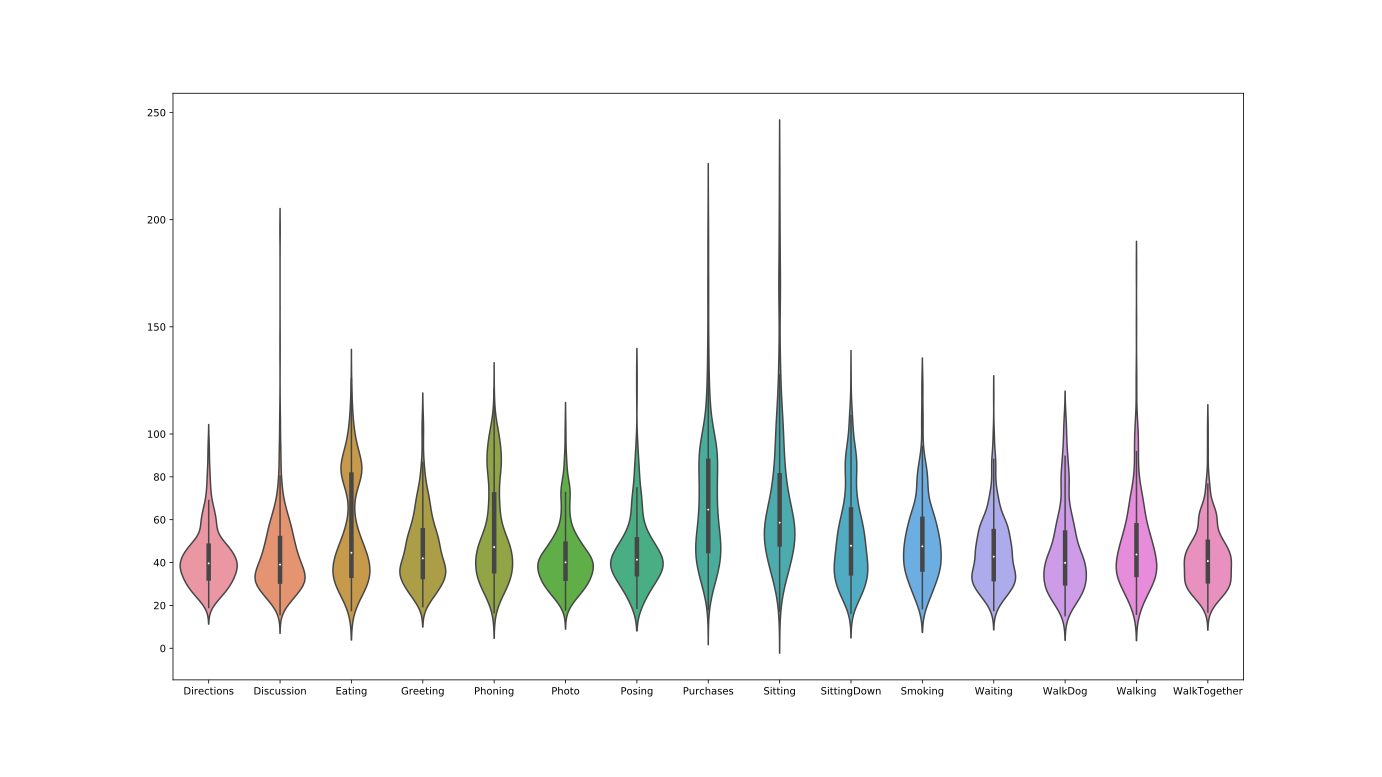
\includegraphics[width=\textwidth]{figures/results/violin_pjpe.pdf}
    \caption{Visualization of the MPJPE error distribution under Protocol $\#2$ for each action.}
    \label{fig:mpjpe_trends}
\end{figure}

The \ac{mpjpe} error per joint increases as we move from inner to outer joints. This can be observed in Table \ref{table:pjpe} which shows the average per joint position error. The error in the limb joints is due to the larger variation in their location through out the data compared to joints like the neck or the nose. Moreover, these joints are often occluded by the person's body especially when doing actions such as sitting. The 2D projections a pose from sitting posture is clustered to a smaller region from certain \acp{pov}. This makes it challenging to estimate the scale and depth of each joint and leads to outliers as visualized in the violin plots.

Since the data consists an equal mix of data from different \acp{pov}, the predictions from the \ac{pov}, where the limbs are in the \ac{fov} are more informative than the other \acp{pov}. When the limbs are not in the \ac{fov}, the model learns to guess their location based on other features such as articulation or posture of the body. The effect of \ac{pov} is the possible cause of the bimodal error distribution in actions such as purchases, eating, phoning. Since the actions are hands specific, they are restricted to a particular region making the pose more predictable from one \ac{pov} and less from another. These challenges are inherent to the task of pose lifting and in many cases is challenging even for a human eye.

\section{Qualitative Results}

\newcommand{\inp}[1]{figures/zv_mean/#1_inp.png}
\newcommand{\pred}[1]{figures/zv_mean/#1_pred.png}
\newcommand{\gt}[1]{figures/zv_mean/#1_gt.png}



\begin{figure}[h]
    \centering
    \begin{subfigure}[b]{0.3\textwidth}
        \includegraphics[width=0.3\textwidth]{\inp{3493}}
        \includegraphics[width=0.3\textwidth]{\pred{3493}}
        \includegraphics[width=0.3\textwidth]{\gt{3493}}
        \caption*{Directions - 44.44mm}
    \end{subfigure}
    \begin{subfigure}[b]{0.3\textwidth}
        \includegraphics[width=0.3\textwidth]{\inp{6422}}
        \includegraphics[width=0.3\textwidth]{\pred{6422}}
        \includegraphics[width=0.3\textwidth]{\gt{6422}}
        \caption*{Discussion - 44.49mm}
    \end{subfigure}
    \begin{subfigure}[b]{0.3\textwidth}
        \includegraphics[width=0.3\textwidth]{\inp{14027}}
        \includegraphics[width=0.3\textwidth]{\pred{14027}}
        \includegraphics[width=0.3\textwidth]{\gt{14027}}
        \caption*{Eating - 56.63mm}
    \end{subfigure}
    \hfill
    \hfill
    \begin{subfigure}[b]{0.3\textwidth}
        \includegraphics[width=0.3\textwidth]{\inp{74176}}
        \includegraphics[width=0.3\textwidth]{\pred{74176}}
        \includegraphics[width=0.3\textwidth]{\gt{74176}}
        \caption*{Greeting - 49.15mm}
    \end{subfigure}
    \begin{subfigure}[b]{0.3\textwidth}
        \includegraphics[width=0.3\textwidth]{\inp{21621}}
        \includegraphics[width=0.3\textwidth]{\pred{21621}}
        \includegraphics[width=0.3\textwidth]{\gt{21621}}
        \caption*{Phoning - 56.59mm}
    \end{subfigure}
    \begin{subfigure}[b]{0.3\textwidth}
        \includegraphics[width=0.3\textwidth]{\inp{26692}}
        \includegraphics[width=0.3\textwidth]{\pred{26692}}
        \includegraphics[width=0.3\textwidth]{\gt{26692}}
        \caption*{Photo - 44.22mm}
    \end{subfigure}
    \hfill
    \hfill
    \begin{subfigure}[b]{0.3\textwidth}
        \includegraphics[width=0.3\textwidth]{\inp{30089}}
        \includegraphics[width=0.3\textwidth]{\pred{30089}}
        \includegraphics[width=0.3\textwidth]{\gt{30089}}
        \caption*{Posing - 46.50mm}
    \end{subfigure}
    \begin{subfigure}[b]{0.3\textwidth}
        \includegraphics[width=0.3\textwidth]{\inp{33987}}
        \includegraphics[width=0.3\textwidth]{\pred{33987}}
        \includegraphics[width=0.3\textwidth]{\gt{33987}}
        \caption*{Purchases - 71.16mm}
    \end{subfigure}
    \begin{subfigure}[b]{0.3\textwidth}
        \includegraphics[width=0.3\textwidth]{\inp{39416}}
        \includegraphics[width=0.3\textwidth]{\pred{39416}}
        \includegraphics[width=0.3\textwidth]{\gt{39416}}
        \caption*{Sitting - 72.55mm}
    \end{subfigure}
    \hfill
    \hfill
    \begin{subfigure}[b]{0.3\textwidth}
        \includegraphics[width=0.3\textwidth]{\inp{94650}}
        \includegraphics[width=0.3\textwidth]{\pred{94650}}
        \includegraphics[width=0.3\textwidth]{\gt{94650}}
        \caption*{SittingDown - 55.01mm}
    \end{subfigure}
    \begin{subfigure}[b]{0.3\textwidth}
        \includegraphics[width=0.3\textwidth]{\inp{96348}}
        \includegraphics[width=0.3\textwidth]{\pred{96348}}
        \includegraphics[width=0.3\textwidth]{\gt{96348}}
        \caption*{Smoking - 51.98mm}
    \end{subfigure}
    \begin{subfigure}[b]{0.3\textwidth}
        \includegraphics[width=0.3\textwidth]{\inp{54005}}
        \includegraphics[width=0.3\textwidth]{\pred{54005}}
        \includegraphics[width=0.3\textwidth]{\gt{54005}}
        \caption*{Waiting - 47.79mm}
    \end{subfigure}
    \hfill
    \hfill
    \begin{subfigure}[b]{0.3\textwidth}
        \includegraphics[width=0.3\textwidth]{\inp{55495}}
        \includegraphics[width=0.3\textwidth]{\pred{55495}}
        \includegraphics[width=0.3\textwidth]{\gt{55495}}
        \caption*{WalkDog - 46.86mm}
    \end{subfigure}
    \begin{subfigure}[b]{0.3\textwidth}
        \includegraphics[width=0.3\textwidth]{\inp{106863}}
        \includegraphics[width=0.3\textwidth]{\pred{106863}}
        \includegraphics[width=0.3\textwidth]{\gt{106863}}
        \caption*{Walking - 48.73mm}
    \end{subfigure}
    \begin{subfigure}[b]{0.3\textwidth}
        \includegraphics[width=0.3\textwidth]{\inp{109473}}
        \includegraphics[width=0.3\textwidth]{\pred{109473}}
        \includegraphics[width=0.3\textwidth]{\gt{109473}}
        \caption*{WalkTogether - 44.00mm}
    \end{subfigure}

    \caption{Left to right are the input 2D poses with RGB reference, the predicted 3D pose (in blue) and the ground truth 3D pose (in pink). The aligned predictions are the ones closest to the mean MPJPE error of every action.}
    \label{fig:zv}
\end{figure}




















% \newcommand{\inp}[1]{figures/zv_fail/fails_#1_inp.png}
\newcommand{\pred}[1]{figures/zv_fail/fails_#1_pred.png}
\newcommand{\gt}[1]{figures/zv_fail/fails_#1_gt.png}


\begin{figure}[h]
    \centering
    \begin{subfigure}[b]{0.45\textwidth}
        \includegraphics[width=0.3\textwidth]{\inp{2878}}
        \includegraphics[width=0.3\textwidth]{\pred{2878}}
        \includegraphics[width=0.3\textwidth]{\gt{2878}}
        % \caption*{Directions - 44.44mm}
    \end{subfigure}
    \begin{subfigure}[b]{0.45\textwidth}
        \includegraphics[width=0.3\textwidth]{\inp{6130}}
        \includegraphics[width=0.3\textwidth]{\pred{6130}}
        \includegraphics[width=0.3\textwidth]{\gt{6130}}
        % \caption*{Discussion - 44.49mm}
    \end{subfigure}



    \begin{subfigure}[b]{0.45\textwidth}
        \includegraphics[width=0.3\textwidth]{\inp{73047}}
        \includegraphics[width=0.3\textwidth]{\pred{73047}}
        \includegraphics[width=0.3\textwidth]{\gt{73047}}
        % \caption*{Eating - 56.63mm}
    \end{subfigure}
    \begin{subfigure}[b]{0.45\textwidth}
        \includegraphics[width=0.3\textwidth]{\inp{18120}}
        \includegraphics[width=0.3\textwidth]{\pred{18120}}
        \includegraphics[width=0.3\textwidth]{\gt{18120}}
        % \caption*{Greeting - 49.15mm}
    \end{subfigure}



    \begin{subfigure}[b]{0.45\textwidth}
        \includegraphics[width=0.3\textwidth]{\inp{24801}}
        \includegraphics[width=0.3\textwidth]{\pred{24801}}
        \includegraphics[width=0.3\textwidth]{\gt{24801}}
        % \caption*{Phoning - 56.59mm}
    \end{subfigure}
    \begin{subfigure}[b]{0.45\textwidth}
        \includegraphics[width=0.3\textwidth]{\inp{26722}}
        \includegraphics[width=0.3\textwidth]{\pred{26722}}
        \includegraphics[width=0.3\textwidth]{\gt{26722}}
        % \caption*{Photo - 44.22mm}
    \end{subfigure}



    \begin{subfigure}[b]{0.45\textwidth}
        \includegraphics[width=0.3\textwidth]{\inp{31669}}
        \includegraphics[width=0.3\textwidth]{\pred{31669}}
        \includegraphics[width=0.3\textwidth]{\gt{31669}}
        % \caption*{Posing - 46.50mm}
    \end{subfigure}
    % \begin{subfigure}[b]{0.45\textwidth}
    %     \includegraphics[width=0.3\textwidth]{\inp{34930}}
    %     \includegraphics[width=0.3\textwidth]{\pred{34930}}
    %     \includegraphics[width=0.3\textwidth]{\gt{34930}}
    % \caption*{Purchases - 71.16mm}
    % \end{subfigure}
    % \begin{subfigure}[b]{0.45\textwidth}
    %     \includegraphics[width=0.3\textwidth]{\inp{90950}}
    %     \includegraphics[width=0.3\textwidth]{\pred{90950}}
    %     \includegraphics[width=0.3\textwidth]{\gt{90950}}
    %     % \caption*{Sitting - 72.55mm}
    % \end{subfigure}
    \begin{subfigure}[b]{0.45\textwidth}
        \includegraphics[width=0.3\textwidth]{\inp{43450}}
        \includegraphics[width=0.3\textwidth]{\pred{43450}}
        \includegraphics[width=0.3\textwidth]{\gt{43450}}
        % \caption*{SittingDown - 55.01mm}
    \end{subfigure}



    \begin{subfigure}[b]{0.45\textwidth}
        \includegraphics[width=0.3\textwidth]{\inp{98756}}
        \includegraphics[width=0.3\textwidth]{\pred{98756}}
        \includegraphics[width=0.3\textwidth]{\gt{98756}}
        % \caption*{Smoking - 51.98mm}
    \end{subfigure}
    \begin{subfigure}[b]{0.45\textwidth}
        \includegraphics[width=0.3\textwidth]{\inp{101351}}
        \includegraphics[width=0.3\textwidth]{\pred{101351}}
        \includegraphics[width=0.3\textwidth]{\gt{101351}}
        % \caption*{Waiting - 47.79mm}
    \end{subfigure}



    \begin{subfigure}[b]{0.45\textwidth}
        \includegraphics[width=0.3\textwidth]{\inp{105002}}
        \includegraphics[width=0.3\textwidth]{\pred{105002}}
        \includegraphics[width=0.3\textwidth]{\gt{105002}}
        % \caption*{WalkDog - 46.86mm}
    \end{subfigure}
    \begin{subfigure}[b]{0.45\textwidth}
        \includegraphics[width=0.3\textwidth]{\inp{106047}}
        \includegraphics[width=0.3\textwidth]{\pred{106047}}
        \includegraphics[width=0.3\textwidth]{\gt{106047}}
        % \caption*{Walking - 48.73mm}
    \end{subfigure}


    \begin{subfigure}[b]{0.45\textwidth}
        \includegraphics[width=0.3\textwidth]{\inp{61221}}
        \includegraphics[width=0.3\textwidth]{\pred{61221}}
        \includegraphics[width=0.3\textwidth]{\gt{61221}}
        % \caption*{WalkTogether - 44.00mm}
    \end{subfigure}

    \caption{Left to right are the input 2D poses with RGB reference, the predicted 3D pose (in blue) and the ground truth 3D pose (in pink). The aligned predictions are the ones closest to the mean MPJPE error of every action.}
    \label{table:zv_fail}
\end{figure}



















\begin{figure}[h]
    \centering
    \includegraphics[width=\textwidth]{example-grid-100x100pt}
    \caption{(a) Prediction on hard poses with hih ambiguity. (b) Poses that can be improved with changes to data processing.}
    \label{fig:bad_samples}
\end{figure}



Some of such outliers are presented in fig \ref{fig:bad_samples}, the predictions in (a) are the ones the model is unable to learn. While (b) is the evidence of the shortcoming of the current processing technique. Rectifying that would improve the evaluation metric of the model quite significantly.



\section{Latent Space}

% begin{figure}[h]
% \centering
%     \includegraphics[width=\textwidth]{figures/results/umap.pdf}
%     \caption{ UMAP Visualization of samples in latent space. The actions do not always directly related to the pose due to overlaps from one action to another. Better viewed in color and zoomed}
% \label{fig:latentspace}
% \end{figure}

% kneeling
7817
0.781
7742
0.940
7123
0.975
6102
0.986
7752
1.025
5484
1.035



half sitting
3418
0.387
2850
0.496
6441
0.644
3279
0.646
7194
0.905
7126
1.001

sitting down
7126
0.848
7264
0.925
7254
0.940
7386
1.028
7237
1.038
7108
1.046

all sitting down
7043
0.422
3079
0.434
2895
0.450
3125
0.641
2888
0.654
2909
0.823


bending
791
0.477
5617
0.591
6755
0.603
826
0.727
629
0.748
8435
0.855


hand motion
5850
0.700
8051
0.724
7614
0.802
7924
0.805
516
0.835
8070
0.836



The visualization of 2D pose embedding in latent space after dimensionality reduction using \ac{umap} is shown in fig. \ref{fig:latentspace}. Each action is given a unique color. Though we small clusters of blues, browns, pinks the overall space looks very mixed up. This is expected as many of the instances in different actions overlap. For example, the action standing up and sitting down have instances while both or standing or sitting, etc.



% \section{missing joints}

\chapter{Conclusions}
\label{chap:conclusions}

\section{Discussion}
%FIXME c3dpo is weakly supervised
%FIXME include new amazon paper somewhere
Previous unsupervised learning approaches for pose lifting such as \cite{amazon1} uses deep neural networks and geometric consistency to achieve results comparable to major weakly supervised approaches such as \cite{can3dpose}. They address critical problems such as making use of datasets from different distribution using additional domain adaptation networks and exploiting temporal information. These techniques made it possible to use large amounts of 2D data to learn 3D poses. However, as the authors acknowledge the \ac{sota} 2D pose networks often get few joints very wrong or miss them due to occlusions that are quite frequent in the real-world. Hence methods that are independent of the correctness of the input 2D are essential. \cite{c3dpo,weaklymultiple} are such weakly supervised methods that can handle missing joints while \cite{weaklymultiple} can also give multiple hypotheses for a given 2D pose. The proposed method tackles these problems with a unified approach by using \acp{vae} and \ac{gan} and is completely unsupervised.

The average \ac{mpjpe} using ZV, 52.74mm, is equivalent to the settings of \cite{amazon1} without additional data or temporal information, 58 mm. This is a significant improvement considering that the network is independent of the input and can handle errors including missing joints, can produce multiple hypotheses. While \cite{amazon1} uses a self-symmetry technique that requires propagating through the models twice per iteration and requires 2 more additional networks of complexity similar to the lifting network to slightly exceed the performance of the proposed network.

Though the proposed network address all the 3 major challenges of lifting networks, i.e 3D annotations, missing joints, and variational inference, the network only predicts a unit 3D pose. This restriction limits the usability of the 3D pose in some cases or requires additional algorithms to obtain the true scale in the real-world. For example, the scale of the 3D pose is not important if the task is to use the method as a vision-based \ac{mocap} solution for gaming where only the articulation of the pose is of interest to capture complex human motion. While tasks in the domain of self-driving cars, robot-human interaction, or AR/VR applications where the pose is used for interaction among the agents, 3D pose alone would not be sufficient.


\section{Future Work}

The source of the major drawback of not predicting to scale is in the processing technique to make the self-supervision simple. This problem could be addressed by extending the method to disentangle the root-relative pose prediction and global pose prediction similar to \cite{CameraDistanceAware}. 

\acp{vae} have more to offer than just predict 3D while handling erroneous inputs. Taking the inspiration from \cite{crossmodal}, the method can be upgraded from a lifting network to end to end network to predict 3D pose from Images just by swapping the encoder model. Techniques like Synergy and Cross-Generation from cross-modal training \cite{MMVAE} could be leveraged to train an unsupervised Image to 3D model faster and efficiently with the help of large 2D pose datasets.

In addition to this guaranteed improvised techniques such as using external datasets and temporal information to learn predicting temporally consistent 3D pose as presented in \cite{amazon1} would make the network more practical to use in the real world.

\section{Final Words}

Scaling the task of 3D Human Pose Estimation to the real-world is limited by the need for 3D data. This thesis presented an unsupervised learning method that learns to predict 3D pose without a need for 3D annotations in any shape or form. The method learns to lift 2D poses to 3D strictly using 2D pose data that are obtained from 2D pose estimation models. The thesis introduced standards \acp{vae} to the task of pose lifting for the first time. This generative model is trained using \ac{gan} and self-supervision techniques. The ability of the proposed method to handle incomplete and erroneous data without explicit training is shown. The thesis also shows the capacity of the model to learn a strong representation of the pose that could be used for other applications such as human-centric multi-view video synchronization. This thesis has considerably improved the \ac{sota} in unsupervised 3D Human Pose Estimation and lays the foundation for new ways to tackle the problem.





\include{content}

\newpage
\addcontentsline{toc}{chapter}{References}
\printbibliography

\newpage
\appendix
\newpage
\etocdepthtag.toc{mtappendix}
\etocsettagdepth{mtchapter}{none}
\etocsettagdepth{mtappendix}{subsection}
\etoctocstyle{1}{Appendix - Contents}
\tableofcontents
\newpage


\chapter{Model Summaries}



\begin{center}
    \begin{tabular}{ p{0.2\textwidth}| p{0.7\textwidth}| p{0.1\textwidth}}

        \textbf{Layer Type)} & \textbf{Output Shape}                                   & \textbf{Parameters} \\
        \hline

        (0):                 & Linear(in features=32, out features=1024, bias=True)    & 33792               \\
        (1):                 & BatchNorm1d(1024, eps=1e-05, momentum=0.1)              & 2048                \\
        (2):                 & Mish()                                                  & 0                   \\
        (3):                 & Dropout(p=0.2, inplace=False)                           & 0                   \\

        (LBAD 1):            & LBAD(                                                   &                     \\

        (w1):                & Linear(in features=1024, out features=1024, bias=False) & 1048576             \\
        (bn1):               & BatchNorm1d(1024, eps=1e-05, momentum=0.1)              & 2048                \\
        (activ):             & Mish()                                                  & 0                   \\
        (dropout):           & Dropout(p=0.2, inplace=False)                           & 0                   \\

        (LBAD 2):            & LBAD(                                                   &                     \\

        (w1):                & Linear(in features=1024, out features=1024, bias=False) & 1048576             \\
        (bn1):               & BatchNorm1d(1024, eps=1e-05, momentum=0.1)              & 2048                \\
        (activ):             & Mish()                                                  & 0                   \\
        (dropout):           & Dropout(p=0.2, inplace=False)                           & 0                   \\

        (downsample):        & LBAD(                                                   &                     \\

        (fc mean):           & Linear(in features=1024, out features=51, bias=True)    & 52275               \\
        (fc logvar):         & Linear(in features=1024, out features=51, bias=True)    & 52275               \\
    \end{tabular}
\end{center}

\begin{center}
    \begin{tabular}{ p{0.2\textwidth}| p{0.7\textwidth}| p{0.1\textwidth}}

        \textbf{Layer Type)} & \textbf{Output Shape}                                                             & \textbf{Parameters} \\
        \hline

        (0):                 & Linear(in features=51, out features=1024, bias=True)                              & 53248               \\
        (1):                 & BatchNorm1d(1024, eps=1e-05, momentum=0.1, affine=True, track running stats=True) & 2048                \\
        (2):                 & Mish()                                                                            & 0                   \\
        (3):                 & Dropout(p=0.2, inplace=False)                                                     & 0                   \\

        (LBAD 1):            & LBAD(                                                                             &                     \\
        (w1):                & Linear(in features=1024, out features=1024, bias=False)                           & 1048576             \\
        (bn1):               & BatchNorm1d(1024, eps=1e-05, momentum=0.1, affine=True, track running stats=True) & 2048                \\
        (activ):             & Mish()                                                                            & 0                   \\
        (dropout):           & Dropout(p=0.2, inplace=False)                                                     & 0                   \\

        (LBAD 2):            & LBAD(                                                                             & 0                   \\
        (w1):                & Linear(in features=1024, out features=1024, bias=False)                           & 1048576             \\
        (bn1):               & BatchNorm1d(1024, eps=1e-05, momentum=0.1, affine=True, track running stats=True) & 2048                \\
        (activ):             & Mish()                                                                            & 0                   \\
        (dropout):           & Dropout(p=0.2, inplace=False)                                                     & 0                   \\

        (dec out block):     & Sequential(                                                                       & 0                   \\
        (0):                 & Linear(in features=1024, out features=48, bias=True)                              & 49200               \\
        (1):                 & Tanh()                                                                            & 0                   \\
    \end{tabular}
\end{center}





\begin{center}
    \begin{tabular}{ p{0.2\textwidth}| p{0.7\textwidth}| p{0.1\textwidth}}

        \textbf{Layer Type)} & \textbf{Output Shape}                                  & \textbf{Parameters} \\
        \hline


        (0):                 & Linear(in features=32, out features=1024, bias=True)   & 33792               \\
        (1):                 & LeakyReLU(negative slope=0.01)                         & 0                   \\

        (LBAD 1):            & LBAD(                                                  &                     \\
        (w1):                & Linear(in features=1024, out features=1024, bias=True) & 1049600             \\
        (activ):             & LeakyReLU(negative slope=0.01)                         & 0                   \\
        (dropout):           & Dropout(p=0.5, inplace=False)                          & 0                   \\

        (LBAD 2):            & LBAD(                                                  & 0                   \\
        (w1):                & Linear(in features=1024, out features=1024, bias=True) & 1049600             \\
        (activ):             & LeakyReLU(negative slope=0.01)                         & 0                   \\
        (dropout):           & Dropout(p=0.5, inplace=False)                          & 0                   \\

        (LBAD 3):            & LBAD(                                                  & 0                   \\
        (w1):                & Linear(in features=1024, out features=1024, bias=True) & 1049600             \\
        (activ):             & LeakyReLU(negative slope=0.01)                         & 0                   \\
        (dropout):           & Dropout(p=0.5, inplace=False)                          & 0                   \\

        (LBAD 4):            & LBAD(                                                  & 0                   \\
        (w1):                & Linear(in features=1024, out features=1024, bias=True) & 1049600             \\
        (activ):             & LeakyReLU(negative slope=0.01)                         & 0                   \\
        (dropout):           & Dropout(p=0.5, inplace=False)                          & 0                   \\

        (out block):         & Sequential(                                            & 0                   \\
        (0):                 & Linear(in features=1024, out features=1, bias=True)    & 1025                \\
        (1):                 & Sigmoid()                                              & 0                   \\
    \end{tabular}
\end{center}



\includepdf[pages=1]{setup/diva-info}

\includepdf[pages=1]{setup/cover-back}

\end{document}


